\documentclass[titlepage]{article}


\usepackage[swedish]{babel}
\usepackage{hyperref}
\usepackage{amsmath, amssymb, amsthm, mathtools}
\usepackage{enumitem}
\usepackage{blindtext}
\usepackage{tcolorbox}
\usepackage{graphicx}
\usepackage{float}
\usepackage{caption}
\usepackage{graphicx}

\definecolor{green}{cmyk}{0.37, 0, 0.94, 0.21, 0.20}

\bibliographystyle{plainurl}



\begin{document}


%% Titelsida
\begin{titlepage}
\begin{center}
    \Huge Att skriva matematik 
    \vspace{2mm}

    \noindent \Large - En introduktion -
    \vfill

    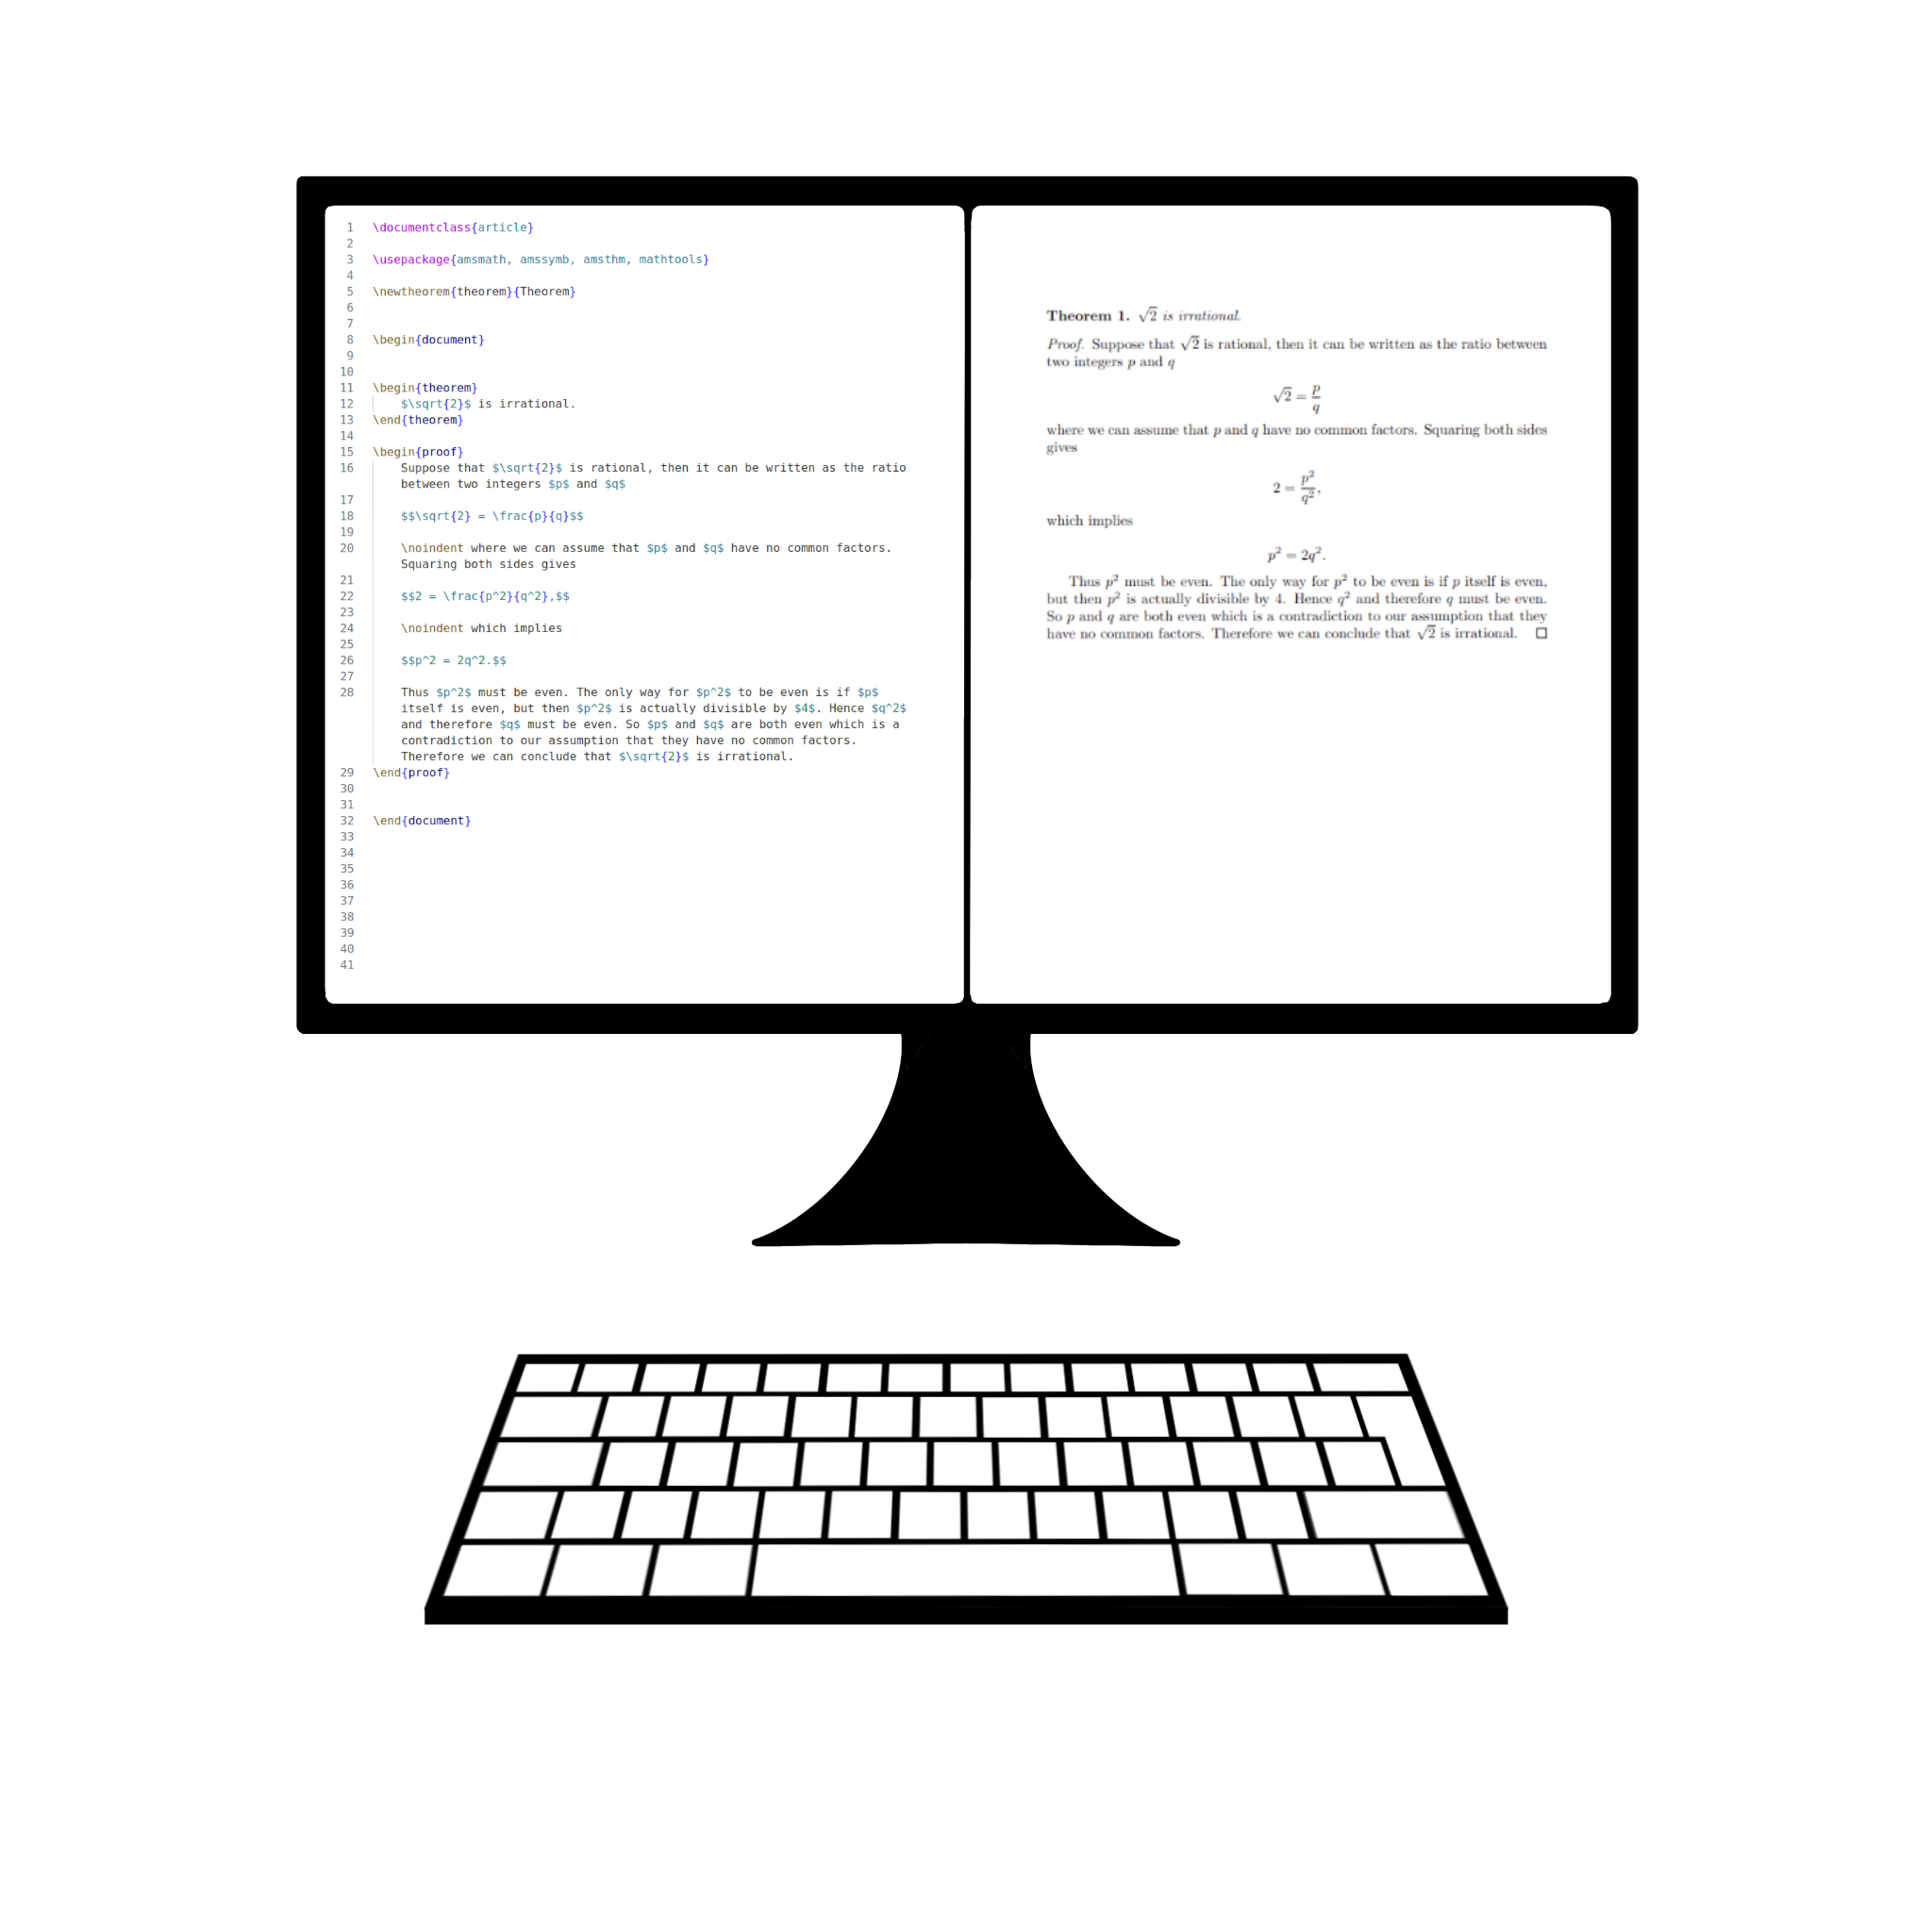
\includegraphics[width = \linewidth]{frontv2.png}
    \vfill
    \Large
    Caroline Roos
\end{center}    
\end{titlepage}


%% TOC
\tableofcontents
\thispagestyle{empty}

\newpage
\setcounter{page}{1}



%%%%%%%%%%%%%%%%%
%%  Inledning  %%
%%%%%%%%%%%%%%%%%

\section{Inledning}

På universitet och högskolor är kraven på skriftliga presentationer höga, och det är därmed viktigt att lära sig skriva matematisk text. I detta kompendium ger vi dig tips och råd på hur du skriver matematik på ett snyggt och tydligt sätt. Tanken är att du som student ska kunna använda detta för att skriva både längre och kortare matematiska texter.

Vi lyfter saker som är extra viktiga att tänka på vid skrivandet, och använder exempel för att tydliggöra skillnaden mellan bra och mindre bra matematisk text. För den som tänker fortsätta läsa matematik och är intresserad av att läsa mer om matematiskt skrivande rekommenderas \textit{Mathematical writing} av Franco Vivaldi\cite{vivaldi}, som är inspirationen bakom flera punkter i Avsnitt \ref{ch2} och \ref{ch3}


%%%%%%%%%%%%%%%%%%%%%%%%%%%%%%%
%%  Allmänna skrivtips       %%
%%    - Siffor och symboler  %%
%%%%%%%%%%%%%%%%%%%%%%%%%%%%%%%

\section{Allmänna skrivtips}\label{ch2}

Börja alltid med att skissa på en lösning på problemet separat innan du börjar skriva själva texten. När du väl har en lösning kan du börja fundera på hur du bäst kan presentera den i text. Det finns många sätt att lösa ett problem på, och ännu fler sätt att presentera lösningar på. Till en början har vi några enkla tumregler att hålla koll på:

\begin{itemize}
    \item En text ska vara sammanhängande och bestå av fullständiga meningar.
    \item Formler och matematiska uttryck ska vara del av fullständiga meningar.
    \item Var noga med att börja varje mening med stor bokstav och avsluta med punkt.
    \item Alla beteckningar som införs ska vara tydligt definierade i texten.
\end{itemize}

Utöver dessa punkter är det såklart viktigt att tänka på stavning och grammatik, precis som när vi skriver vilken annan text som helst.



%% Siffor och symboler

\subsection{Siffror och symboler}

Något som kan vara svårt i början är att hitta balansen i att kombinera siffror, symboler och ord. Det är lockande att ofta använda matematiska symboler, men en överanvändning av dessa kan i själva verket göra din text svårläslig. För att undvika detta inför vi ytterligare några tumregler:

\begin{itemize}
    \item Börja inte en mening med en siffra eller symbol om det kan undvikas.
        \begin{itemize}[leftmargin=20mm]
            \item[\textbf{Sämre:}] $\pi$ är ett irrationellt tal.
            \item[\textbf{Bättre:}] Talet $\pi$ är irrationellt. 
        \end{itemize}
    \item En mening innehållandes siffror och symboler måste fortfarande vara en korrekt fullständig mening.
        \begin{itemize}[leftmargin=20mm]
            \item[\textbf{Sämre:}] $a < b \: a \neq 0$
            \item[\textbf{Bättre:}] Vi har att $a<b$ och $a \neq 0$.
            \vspace{2mm}
            \item[\textbf{Sämre:}] $x^2 - 7^2 = 0.\: x = \pm 7$
            \item[\textbf{Bättre:}] Låt $x^2 - 7^2 = 0$, då är $x = \pm 7.$
        \end{itemize}
    \item Blanda inte symboler och ord.
        \begin{itemize}[leftmargin=20mm]
            \item[\textbf{Sämre:}] Differensen $a-b$ är $<0$.
            \item[\textbf{Bättre:}] Differensen $a-b$ är negativ.
        \end{itemize}
    \item Missbruka inte implikationspilen $\Rightarrow$ eller symbolen $\therefore$ .
        \begin{itemize}[leftmargin=20mm]
            \item[\textbf{Sämre:}] $a$ är ett heltal $\Rightarrow a$ är ett rationellt tal.
            \item[\textbf{Bättre:}] Om $a$ är ett heltal så är $a$ ett rationellt tal.
            \vspace{2mm}
            \item[\textbf{Sämre:}] Vi har att $x+5=8 \therefore x = 3$
            \item[\textbf{Bättre:}]  Vi har att $x+5=8$, då följer det att $x = 3$.
        \end{itemize}
\end{itemize}


%%%%%%%%%%%%%%%%%%%%%%%%%%%%%%%%%%%
%%  Notation                     %%
%%    - Aritmetik                %%
%%    - Mängder och intervall    %%
%%%%%%%%%%%%%%%%%%%%%%%%%%%%%%%%%%%


\section{Notation}\label{ch3}

Var försiktig och noggrann med matematisk notation. Se till att du förstår innebörden hos olika symboler innan du använder dem, till exempel betyder olika parenteser (( ), [ ], \{ \}) och pilar ($\Rightarrow$, $\Leftrightarrow$, $\to$) olika saker. Fel symbol kan göra att det du skriver inte är matematiskt korrekt, eller att du skriver någonting annat än det du faktiskt menar.



%% Aritmetik

\subsection{Aritmetik}

Notationen för de aritmetiska operationerna är välbekanta sedan grundskolan. Summa och differens av två tal $x$ och $y$ skrivs alltid som $x+y$ respektive $x-y$. Däremot finns det flera sätt att skriva produkten av $x$ och $y$:
$$xy, \hspace{10mm} x\cdot y, \hspace{10mm} x \times y,$$
och samma sak när det kommer till deras kvot:
$$\frac{x}{y}, \hspace{10mm} x/y, \hspace{10mm}  x : y.$$
Notationen $x:y$ är inte särskilt vanlig, och kan betyda olika saker i olika sammanhang, så vi undviker att använda denna. Det vanligaste är att använda $xy$ eller $x \cdot y$ för multiplikation, samt $\frac{x}{y}$ och $x/y$ för division, därför rekommenderar vi att du också gör det. Använd aldrig punkt '.' eller bokstaven 'x' för att uttrycka en produkt, detta leder direkt till förvirring hos läsaren.




%% Mängder och intervall

\subsection{Mängder och intervall}

Ett intervall är en delmängd av de rella talen av typen
$$[a,b] := \{x \in \mathbb{R}\: : \: a\leq x \leq b\}$$
där $a,b$ är rella tal och $a<b$. Det här är ett slutet intervall, vilket innebär att det innehåller ändpunkterna. Vi kan också definiera öppna intervall 
$$(a,b) := \{x \in \mathbb{R} \: : \: a<x<b\}$$
och halvöppna intervall
$$[a,b) \hspace{10mm} \text{och} \hspace{10mm}(a,b].$$

Notationen för det öppna intervallet krockar med notationen för ett ordnat par $(a,b) \in \mathbb{R}^2$ som man brukar använda för att till exempel uttrycka en punkt i ett koordinatsystem. Det finns alternativa sätt att uttrycka öppna och halvöppna intervall på
$$]a,b[, \hspace{10mm} [a,b[, \hspace{10mm} ]a,b],$$
men så länge det framgår tydligt från kontexten att det är ett intervall vi syftar på så fungerar båda notationerna lika bra.

Ibland vill vi uttrycka intervall som sträcker sig mot oändligheten. Säg att vi vill ange värdemängden till funktionen $f(x) = x^2$. Denna består som bekant av alla icke-negativa reella tal och vi kan uttrycka den med mängdnotation
$$\{ a \: : \: 0 \leq a < \infty \},$$
eller med notationen för intervall
$$[0, \infty[.$$

Notera att vi använt oss av strikt olikhet och öppet intervall här då $\infty$ inte är ett tal och därför inte kan antas av funktionen.



%% Decimaltal

\subsection{Decimaltal}

I grundskolan lär vi oss att skriva decimaltal med kommatecken (till exempel $1,5$), men detta visar sig dock vara problematiskt då vi använder kommatecknet för att bland annat separera element i mängder. Därför använder vi oss av punkt istället. Låt oss definiera mängden $A$ bestående av tre decimaltal
$$A = \{0.1,2.3,4.5\}.$$

Hade vi istället använt kommatecken i decimaltal hade samma mängd sett ut så här
$$A = \{0,1,2,3,4,5\},$$
men det här är ju mängden som innehåller alla heltal från $0$ till $5$, inte de tre decimaltalen vi definierade mängden med.

I de allra flesta fall är det bäst att hålla sig till att skriva talen på bråkform. På så sätt är talen alltid exakta och lättare att räkna med.



%%%%%%%%%%%%%%%%%%%%%
%%  Struktur       %%
%%%%%%%%%%%%%%%%%%%%%

\section{Struktur}

Oavsett om du skriver en uppsats eller en lösning till en inlämningsuppgift så behöver texten vara strukturerad på ett lämpligt sätt. Det ska vara enkelt för läsaren att följa och förstå det du har gjort. 

\begin{itemize}[leftmargin=25mm, rightmargin=0mm]
    \item[\textbf{Inledning:}] Börja med att beskriva problemet som ska lösas och ange vilka metoder som används, samt varför vi kan tillämpa dessa.
    \item[\textbf{Huvudtext:}] Här skriver du själva lösningen på problemet. Se till att dina logiska argument är lätta att följa, och motivera alla steg i din lösning. Tänk på tumreglerna från Avsnitt \ref{ch2} och var var noga med notationen.
    \item[\textbf{Slutsats:}] Avsluta alltid med en slutsats där du sammanfattar vad du kom fram till.
\end{itemize}

Det kan vara så att en inledning inte alltid är strikt nödvändig, till exempel på en läxa, men det beror på problemet och hur lång och komplex lösningen är. Det är en god vana att ändå alltid skriva åtminstone en inledande mening eller två.



%%%%%%%%%%%%%%%%%%%%%%%%%%%
%%  Typsättning i LaTeX  %%
%%%%%%%%%%%%%%%%%%%%%%%%%%%

\section{Typsättning i \LaTeX}

Det finns inget formellt krav på att använda \LaTeX$ $ i kursen, men det är starkt rekommenderat. Att skriva \LaTeX-kod är enkelt, du omger bara det matematiska uttrycket med dollartecken. Till exempel renderas \LaTeX-koden \$1+x=5\$ som $1+x=5$. Om du vill att det matematiska uttrycket ska stå skrivet på en egen rad så omger du det istället med dubbla dollartecken, då får vi att \$\$1+x=5\$\$ renderas som $$1+x=5.$$

Fördelen med att typsätta i \LaTeX$ $ är att vi kan skriva matematik på ett snyggt och lättläst vis. Vi kan skriva alla matematiska symboler som vi normalt använder med \LaTeX-kod, dessa är vanligtvis svåra att uttrycka i ett vanligt ordbehandlingsprogram. I Tabell \ref{t1} och \ref{t2} finns exempel på hur vanliga matematiska symboler och uttryck kan skrivas i \LaTeX. Exempel på lite mer komplicerade uttryck och hur dessa skrivs i \LaTeX$ $ återfinns i Tabell \ref{t3}.

\begin{table}
\begin{minipage}[b]{.5\linewidth}
    \begin{center}
    \begin{tabular}{| c | l |}
        \hline 
        \textbf{Rendering} & \textbf{\LaTeX-kod} \\
        \hline
        $\pi$ & \$ \textbackslash pi \$ \\
        \hline
        $\sqrt{ x }$ & \$ \textbackslash sqrt\{x\} \$ \\
        \hline
        $\equiv$ & \$ \textbackslash equiv \$ \\
        \hline
        $\cdot$ & \$ \textbackslash cdot \$ \\
        \hline
        $\mathbb{R}$ & \$ \textbackslash mathbb\{R\} \$ \\
        \hline
        $\implies$ & \$ \textbackslash implies \$ \\
        \hline
        $\pm$ & \$ \textbackslash pm \$ \\
        \hline
        $\leq$ & \$ \textbackslash leq \$ \\
        \hline
        $\geq$ & \$ \textbackslash geq \$ \\
        \hline
        $\neq$ & \$ \textbackslash neq \$ \\
        \hline
        $\infty$ & \$ \textbackslash infty \$ \\
        \hline
    \end{tabular}
    \caption{Vanliga symboler i \LaTeX.}
    \label{t1}
    \end{center}
\end{minipage}
\begin{minipage}[b]{.5\linewidth}
    \begin{center}
        \begin{tabular}{| l | l |}
            \hline
            \textbf{Rendering} & \textbf{\LaTeX-kod} \\
            \hline
            $a+b$ & \$ a+b \$ \\
            \hline
            $a-b$ & \$ a-b \$ \\
            \hline
            $a \cdot b$ & \$ a \textbackslash cdot b \$ \\
            \hline
            $\frac{a}{b}$ & \$ \textbackslash frac\{a\}\{b\} \$ \\
            \hline
            $a^b$ & \$ a\textasciicircum b \$ \\
            \hline
            $f(x)$ & \$ f(x) \$ \\
            \hline
            $\sin(v)$ & \$ \textbackslash sin(v) \$ \\
            \hline
        \end{tabular}
        \caption{Vanliga uttryck i \LaTeX.}
        \label{t2}
    \end{center}
\end{minipage}
\end{table}

\begin{table}[H]
    \begin{center}
        \begin{tabular}{| l | l |}
            \hline
            \textbf{Rendering} & \textbf{\LaTeX-kod} \\
            \hline
            $5+5 \leq 10$ & \$ 5+5 \textbackslash leq 10 \$ \\
            \hline
            $2^{4\cdot3 + 1}$ & \$ 2\textasciicircum \{4 \textbackslash cdot 3 + 1\} \$ \\
            \hline
            $13 \equiv_5 3$ & \$ 13 \textbackslash equiv\_5 3 \$ \\
            \hline
            $\{a,b,c\}$ & \$ \textbackslash\{ a,b,c \textbackslash\} \$ \\
            \hline
            $f:\mathbb{Z}_{+} \to \mathbb{R}$ & \$ f: \textbackslash mathbb\{Z\}\_\{+\} \textbackslash to \textbackslash mathbb\{R\} \$ \\
            \hline
            $p(x)=x^3+5x^2-8x+2$ & \$ p(x)=x\textasciicircum 3+4x\textasciicircum 2-8x+2 \$ \\
            \hline
            $\sin(\pi)+\cos(\pi/2)$ & \$\textbackslash sin(\textbackslash pi)+\textbackslash cos(\textbackslash pi/2)\$ \\
            \hline
            $x_{1,2} = -\frac{7}{2} \pm \sqrt{5}$ & \$ x\_\{1,2\} = -\textbackslash frac\{p\}\{2\} \textbackslash pm \textbackslash sqrt\{5\} \$ \\
            \hline
        \end{tabular}
        \caption{\LaTeX-exempel.}
        \label{t3}
    \end{center}
\end{table}




%%%%%%%%%%%%%%%
%%  Exempel  %%
%%%%%%%%%%%%%%%

\section{Exempel}

Det är dags att ta allt vi lärt oss och använda det för att analysera några exempel.


\subsection*{Exempel 1}

%% Exempel 1
\begin{center}
\begin{tcolorbox}[width=\linewidth,colback={white},title={\textbf{Problem}},outer arc=0mm,colupper=black]
    Faktorisera polynomet $p(x)=x^2-5x+6$.
\end{tcolorbox} 
\end{center}

Studera lösningen nedan och fundera först själv på vad problemet med den är och vad vi kan göra för att förbättra den.

\begin{center}
\begin{tcolorbox}[width=\linewidth,colback={red!15!white},title={\textbf{Lösning 1 - Sämre}},outer arc=0mm,colupper=black]
    $x^2-5x+6 = 0 => x=5/2 \pm$ rotenur$1/4$

    Rötterna är $x_1 = 2$, $x_2 = 3$. Det ger faktoriseringen $(x-2)(x-3)$.
\end{tcolorbox} 
\end{center}

Det finns flera problem med den här lösningen. För det första är den översta raden nästan oläslig, detta skulle vi kunna rätta till genom att använda \LaTeX$\:$ och skriva fullständiga meningar istället för enbart siffror och symboler. Något annat som saknas i denna lösning är motiveringar. Det framgår inte vilken metod som användes för att räkna fram rötterna eller varför vi får just denna faktorisering. Jämför nu med följande lösning.

\begin{center}
\begin{tcolorbox}[width=\linewidth,colback={green!25!white},title={\textbf{Lösning 2 - Bättre}},outer arc=0mm,colupper=black]    
    Vi börjar med att sätta $p(x)=0$ och löser ekvationen genom att kvadratkomplettera:
    \vspace{2mm}

    $\quad \: x^2-5x+6 = 0$

    $\Leftrightarrow x^2-5x = -6$

    $\Leftrightarrow(x-\frac{5}{2})^2 = \frac{1}{4}$
    \vspace{2mm}

    Nu drar vi roten ur båda led:
    \vspace{2mm}

    $\quad \: x-\frac{5}{2} = \pm \sqrt{\frac{1}{4}}$

    $\Leftrightarrow x = \frac{5}{2} \pm \frac{1}{2}$
    \vspace{2mm}

    Detta ger oss lösningarna $x_1 = 2$ och $x_2=3$.

    Enligt faktorsatsen är $(x-a)$ en faktor till polynomet $p(x)$ om och endast om $x = a$ är en rot till $p(x)$. Det följer av satsen, och att ett andragradspolynom inte kan ha fler än två rötter, att $p(x) = (x-2)(x-3)$.
\end{tcolorbox} 
\end{center}

Här inleder vi med att beskriva vad vi ska göra och vi använder \LaTeX$\:$ för att skriva ekvationerna. Notera att vi också ställt upp ekvationerna på ett mer lättläst vis. Det framgår också tydligt med hänvisning till faktorsatsen hur vi kommer fram till faktoriseringen.


%% Exempel 2
\subsection*{Exempel 2}

\begin{center}
\begin{tcolorbox}[width=\linewidth,colback={white},title={\textbf{Problem}},outer arc=0mm,colupper=black]
    Beräkna resten då $2^{156}\cdot5$ delas med $7$.
\end{tcolorbox} 
\end{center}

Ett försök på en lösning skulle kunna se ut som Lösning 1 nedan. Fundera på hur du skulle kunna förbättra denna.

\begin{center}
\begin{tcolorbox}[width=\linewidth,colback={red!15!white},title={\textbf{Lösning 1 - Sämre}},outer arc=0mm,colupper=black]
    Vi använder moduloräkning för att hitta resten.

    2\textasciicircum{156}*5 = (2\textasciicircum2)\textasciicircum 78*5 (mod 7) = 4\textasciicircum78*5 (mod 7) = (4\textasciicircum2)\textasciicircum39*5 (mod 7) = 16\textasciicircum39*5 (mod 7) = 2\textasciicircum39*5 (mod 7) = (2\textasciicircum3)\textasciicircum13*5 (mod 7) = 8\textasciicircum13*5 (mod 7) = 1\textasciicircum13*5 (mod 7) = 1*5 (mod 7) = 5(mod 7)

    Svar: resten är 1
\end{tcolorbox} 
\end{center}

Det första du tänkte på var säkert att det var nästintill omöjligt att läsa och hänga med i uträkningen. Vi gör ett nytt försök och skriver uträkningarna i \LaTeX$\:$ istället.

\begin{center}
\begin{tcolorbox}[width=\linewidth,colback={red!15!white},title={\textbf{Lösning 2 - Något bättre}},outer arc=0mm,colupper=black]
    Vi använder moduloräkning för att hitta resten.

    $2^{156}\cdot 5 \equiv_7 (2^2)^{78}\cdot 5\equiv_7 4^{78} \cdot 5 \equiv_7 (4^2)^{39} \cdot 5 \equiv_7 16^{39} \cdot 5 \equiv_7 2^{39} \cdot 5 \equiv_7 (2^3)^{13} \cdot 5 \equiv_7 1^{13}\cdot 5 \equiv_7 1 \cdot 5 \equiv_7 5$

    Svar: Resten när $2^{156}$ delas på $7$ är $1$.
\end{tcolorbox} 
\end{center}

Nu är det lättare att läsa och följa uträkningen. Men det finns fortfarande en hel del problem med den här lösningen. Trots att uträkningen nu går att läsa så är den väldigt lång och är fortfarande inte att klassa som lättläst. Dessutom har vi använt symbolen $\equiv_7$ i varje steg, även på de platser där det faktiskt är likhet. Detta är tekniskt sett fortfarande korrekt, men det är tydligare om vi skriver likhet där det faktiskt är likhet. 

Mot slutet av räkningarna så framkommer det även att $2^3 \equiv_7 1$, detta bör vi givetvis använda oss av redan från början för att slippa onödigt långa uträkningar.

Sist men inte minst bör vi fundera på om allt i lösningen är tillräckligt motiverat. Vi påstår att vi kan använda moduloräkning för att hitta resten vid division, men det framgår inte varför detta skulle vara fallet. Här krävs det att vi motiverar vårat val av metod.

\begin{center}
    \begin{tcolorbox}[width=\linewidth,colback={green!25!white},title={\textbf{Lösning 3 - Bättre}},outer arc=0mm,colupper=black]
        Om $a$ och $r$ är kongruenta modulo $b$ och $0\leq r<b$, så lämnar $a$ resten $r$ vid division med $b$. Detta gör det möjligt för oss att använda moduloräkning för att hitta resten. \vspace{2mm}

        Vi noterar att $2^3 \equiv_7 1$ och att $156 = 3\cdot 52$. Då kan vi göra omskrivningen $2^{156}\cdot 5 = (2^3)^{52} \cdot 5$ med hjälp av potenslagarna. Det ger oss

        $$2^{156}\cdot 5 = (2^3)^{52} \cdot 5 \equiv_7 1^{52} \cdot 5 = 5$$

        Eftersom $0\leq 5<7$ så kan vi dra slutsatsen att resten då $2^{156}$ divideras med $7$ är $5$.
    \end{tcolorbox} 
    \end{center}

Denna lösning är mycket bättre. Vi har en inledning där vi beskriver hur vi hittar resten och motiverar varför vi kan använda denna metod. Därefter har vi en kort huvudtext där vi löser problemet på ett effektivt sätt och motiverar stegen. Vi avslutar sedan med en kort slutsats.



%%%%%%%%%%%%%%%%
%%  Övningar  %%
%%%%%%%%%%%%%%%%

\section{Övningar}
\begin{enumerate}
    \item Skriv om följande meningar så att de följer tumreglerna för hur man skriver matematisk text:
    \begin{enumerate}[label=(\alph*)]
        \item $x$ är negativ $\therefore \sqrt{x}$ är ett komplext tal.
        \item $x^2 = 4 \Rightarrow x=2 \vee x=-2$.
        \item $a$ är $>0$.
        \item Om $x>0$ $g(x) \neq 0$.
        \item $\sin(\pi x)= 0\Rightarrow x$ är ett heltal. 
    \end{enumerate}
    \item Beskriv följande mängder med ord:
    \begin{enumerate}
        \item $\{x \in \mathbb{Q} \: : \: 0<x<1\}$
        \item $\{x \in \mathbb{Z} \: : \: 0 < x \wedge 2 \mid x\}$
    \end{enumerate}
    \item Förklara utan att använda några matematiska symboler:
    \begin{enumerate}[label=(\alph*)]
        \item Hur dividerar man två bråk med varandra?
        \item Givet ett positivt heltal $x$, hur tar man reda på om $x$ är ett primtal?
        \item Givet ett positivt heltal $x$, hur tar man reda på om $x$ är summan av två kvadrater?
    \end{enumerate}
    \item Förbättra lösningen:
    \begin{enumerate}[leftmargin=20mm]
        \item[Problem:] Hitta alla rötter till polynomet $p(x)=x^3 - 4x^2 - 7x + 10$.
        \item[Lösning:] x=1 är en rot ser vi. polynomdivision ger x\textasciicircum2-3x-10 som har rötterna x=-2 och x=5.
    \end{enumerate}
    Tips: Tänk på strukturen och motivera stegen.
\end{enumerate}




%% References
\newpage
\bibliography{refs}


\end{document}